
\documentclass[a4paper, 12pt]{article}

\usepackage[utf8]{inputenc}
\usepackage[T1, T2A]{fontenc}
\usepackage[english, russian]{babel}

\usepackage[top=2cm, bottom=2.5cm, left=2cm, right=2cm]{geometry}
\usepackage{graphicx}
\usepackage{indentfirst}
\usepackage{pgfplots}
\pgfplotsset{compat=1.13}
\pgfplotsset{grid style={dashed, black}}
\newcommand\tline[2]{$\underset{\text{#1}}{\text{\underline{\hspace{#2}}}}$}
\usepackage{subcaption}

\usepackage{amsmath}

\usepackage{caption} 
\captionsetup[figure]{name = Рисунок, labelsep = endash}
\captionsetup[table]{name = Таблица, labelsep = endash, justification=RaggedRight, singlelinecheck=false}
\renewcommand{\baselinestretch}{1.5} 
\parindent=1.27cm
\usepackage{pdfpages}

\begin{document}

\includepdf{titul}
\paragraph{Цель работы.} Изучение математических моделей и исследование характеристик электромеханического объекта управления, построенного на основе электродвигателя постоянного тока независимого возбуждения
\paragraph{Исходные данные:}\hfill

\begin{table}[h!]
\centering
\renewcommand{\arraystretch}{0.8}
\renewcommand{\tabcolsep}{0.4cm}
\caption{Исходные данные}
\begin{tabular}{|c|c|c|c|c|c|c|c|c|c|}

\hline
Un, & n_0,& In,& Mn, & R, & Tя, & Jд, & Ty,& ip & Jm,\\
В& \text{рад/сек} &А&Нм&Ом& c&кг*м^2&с & & кг*м^2\\
\hline
27 &	255.5162&	0.38&	0.04&	32&	0.006&	0.0000055&	0.003&	40&	0.03\\
\hline
\end{tabular}  

\end{table}
Расчет параметров математической модели:
\begin{gather}
K_y=\frac{U_n}{U_m}=\frac{27}{10}=2.7\\
K_d=\frac{1}{R}=\frac{1}{32}=0.0313 \\
K_m=\frac{M_n}{I_n}=\frac{0.04}{0.38}=0.1053\\
J_p=0.2J_d=0.0000011\\
J_\Sigma=J_d+J_p+\frac{J_m}{i_p^2}=0.0000066+\frac{0.03}{1600}=0.00002535\\
K_e=\frac{U_n}{\omega_0}=\frac{27}{255.5}=0.105668447\\
K=\frac{K_y}{K_e*i_p}=0.63879\\
T_m=\frac{RJ_\Sigma}{K_M*K_E}=0.07265\\
K_f=\frac{R}{K_m*K_e*i_p^2}=1.79118
\end{gather}
\par
\vspace{1cm}
В лабораторной работе исследуется электромеханический объект, функциональная схема которого изображена на рисунке 1. На рисунке 2 - структурная схема системы. Схема моделирования изображена на рисунке 3.\par
\begin{figure}[h!]
\begin{center}
\includegraphics[width=13cm]{emo}
\caption{Функциональная схема ЭМО}
\end{center}  
\end{figure}
\newpage
\begin{figure}[h]
	\begin{center}
		\includegraphics[width=13cm]{stru}
		\caption{Структурная схема системы}
	\end{center}  
\end{figure}
\begin{figure}[h!]
\begin{center}
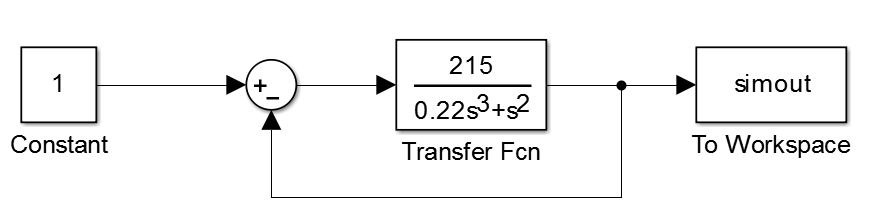
\includegraphics[width=13cm]{schem1}
\caption{Схема моделирования системы}
\end{center}  
\end{figure}
\newpage
Для обеспечения соответствия максимального значения измеряемого сигнала уровню 10 ед., выходной сигнал необходимо домножить на коэффициент передачи:\\
Ky=0.74\\ Ki=28.33\\ Kw=0.078\\ Ka=0.315\\


\newpage


\begin{center}
\section{Получение графиков переходных процессов при нагрузочном моменте 0 Нм и напряжении 5 В}
\end{center}\par
На рисунке 4 изображены графики переходных процессов полной модели ЭМО при холостом ходу. 
\begin{figure}[h]
\begin{minipage}[h]{0.55\linewidth}
\centering{\includegraphics[width=1\linewidth]{Uy1} \\ Uy}
\end{minipage}
\hfill
\begin{minipage}[h]{0.55\linewidth}
\centering{\includegraphics[width=1\linewidth]{I1} \\ I}
\end{minipage}
\vfill
\begin{minipage}[h]{0.55\linewidth}
\centering{\includegraphics[width=1\linewidth]{w1} \\ $\omega$}
\end{minipage}
\hfill
\begin{minipage}[h]{0.55\linewidth}
\centering{\includegraphics[width=1\linewidth]{am1} \\ $\alpha_m$}
\end{minipage}
\caption{Графики переходных процессов при Mcm=0Нм, U=5 В}
\end{figure}
\newpage
\begin{center}
\section{Исследование влияния момента сопротивления на вид переходных процессов}
\end{center}\par
Для исследования влияния момента сопротивления на вид переходных процессов необходимо, оставив все параметры системы неизменными, изменять параметр Mcm от 0 до ip*Mn=1.6. Полученные при исследовании графики изображены на рисунке 5.\\
\begin{figure}[h]
	\begin{minipage}[h]{0.55\linewidth}
		\centering{\includegraphics[width=1\linewidth]{Uy1} \\ Uy}
	\end{minipage}
	\hfill
	\begin{minipage}[h]{0.55\linewidth}
		\centering{\includegraphics[width=1\linewidth]{I2} \\ I}
	\end{minipage}
	\vfill
	\begin{minipage}[h]{0.55\linewidth}
		\centering{\includegraphics[width=1\linewidth]{w2} \\ $\omega$}
	\end{minipage}
	\hfill
	\begin{minipage}[h]{0.55\linewidth}
		\centering{\includegraphics[width=1\linewidth]{am2} \\ $\alpha_m$}
	\end{minipage}
	\caption{Графики переходных процессов при различных Mcm}
\end{figure}\\
Определение установившихся значений:\\
Для I:\\
При M=0Нм, tп=0.3c, Iу=0 A\\
При M=0.5Нм, tп=0.3с, I=3.43*Ki A\\
При M=1Нм, tп=0.3с, I=6.73*Ki A\\
При M=1.6Нм, tп=0.3с, I=10.76*Ki A\\
\newpage\hfill\\
Для $\omega$:\\
При M=0Нм, tп=0.25c,  $\omega$=10*Kw рад/сек\\
При M=0.5Нм, tп=0.25с, $\omega$=7.2*Kw рад/сек\\
При M=1Нм, tп=0.25с, $\omega$=4.4*Kw рад/сек\\
При M=1.6Нм, tп=0.25с, $\omega$=1.06*Kw рад/сек\\
\newpage
\begin{center}
	\section{Исследование влияния момента инерции нагрузки на вид переходных процессов}
\end{center}\par
Графики полученные при исследовании влияния момента инерции нагрузки на вид переходных процессов изображены на рисунке 6.
\begin{figure}[h]
\begin{minipage}[h]{0.55\linewidth}
\centering{\includegraphics[width=1\linewidth]{Uy1} \\ Uy}
\end{minipage}
\hfill
\begin{minipage}[h]{0.55\linewidth}
\centering{\includegraphics[width=1\linewidth]{I3} \\ I}
\end{minipage}
\vfill
\begin{minipage}[h]{0.55\linewidth}
\centering{\includegraphics[width=1\linewidth]{w3} \\ $\omega$}
\end{minipage}
\hfill
\begin{minipage}[h]{0.55\linewidth}
	\centering{\includegraphics[width=1\linewidth]{am3} \\ $\alpha_m$}
\end{minipage}
\caption{Графики переходных процессов при различном Jm}
\end{figure}\\
Определение установившихся значений:\\
Для I:\\
При 0.5Jm, tп=0.2c, Iу=0 A\\
При Jm, tп=0.35с, I=0 A\\
При 1.5Jm, tп=0.5с, I=0 A\\
Для $\omega$:\\
При 0.5Jm, tп=0.2c,  $\omega$=10*Kw рад/сек\\
При Jm, tп=0.3с,$\omega$=10*Kw рад/сек\\
При 1.5Jm, tп=0.4с, $\omega$=10*Kw рад/сек
\newpage
\begin{center}
\section{Исследование влияния передаточного отношения редуктора на вид переходных процессов}
\end{center}\par
Для исследования влияния передаточного отношения редуктора на вид переходных процессов необходимо провести моделирование системы при Mcm=0 и Mcm=0.8Нм. Полученных графики переходных процессов изображены на рисунках 7 и 8.
\begin{figure}[h]
	\begin{minipage}[h]{0.55\linewidth}
		\centering{\includegraphics[width=1\linewidth]{Uy1} \\ Uy}
	\end{minipage}
	\hfill
	\begin{minipage}[h]{0.55\linewidth}
		\centering{\includegraphics[width=1\linewidth]{I4} \\ I}
	\end{minipage}
	\vfill
	\begin{minipage}[h]{0.55\linewidth}
		\centering{\includegraphics[width=1\linewidth]{w4} \\ $\omega$}
	\end{minipage}
	\hfill
	\begin{minipage}[h]{0.55\linewidth}
		\centering{\includegraphics[width=1\linewidth]{am4} \\ $\alpha_m$}
	\end{minipage}
	\caption{Графики переходных процессов при различном ip и Mcm=0 Нм}
\end{figure}
\newpage
\begin{figure}[h]
	\begin{minipage}[h]{0.55\linewidth}
		\centering{\includegraphics[width=1\linewidth]{Uy1} \\ Uy}
	\end{minipage}
	\hfill
	\begin{minipage}[h]{0.55\linewidth}
		\centering{\includegraphics[width=1\linewidth]{I5} \\ I}
	\end{minipage}
	\vfill
	\begin{minipage}[h]{0.55\linewidth}
		\centering{\includegraphics[width=1\linewidth]{w5} \\ $\omega$}
	\end{minipage}
	\hfill
	\begin{minipage}[h]{0.55\linewidth}
		\centering{\includegraphics[width=1\linewidth]{am5} \\ $\alpha_m$}
	\end{minipage}
	\caption{Графики переходных процессов при различном ip и Mcm=0.8 Нм}
\end{figure}
\newpage
\begin{center}
	\section{Анализ погрешности вызванной упрощением модели}
\end{center}\par
Если $T_\text{y}$ и $T_\text{я}$ значительно меньше, чем механическая постоянная времени $T_\text{м}$, то для упрощения математической модели, апериодические звенья можно заменить пропорциональными звеньями с коэффициентами передачи $K_\text{д}$ и $K_\text{у}$. Схема моделирования упрощенной модели изображена на рисунке 9. Сравнения переходных характеристик полной и упрощенной модели - на рисунке 10.
\begin{figure}[h]
\begin{center}
\includegraphics[width=13cm]{scheme2}
\caption{Схема моделирования упрощенной модели}
\end{center}  
\end{figure}

\begin{figure}[h]
\begin{minipage}[h]{0.49\linewidth}
\centering{\includegraphics[width=1\linewidth]{w7} \\ $\omega$}
\end{minipage}
\hfill
\begin{minipage}[h]{0.49\linewidth}
\centering{\includegraphics[width=1\linewidth]{am7} \\ $\alpha_m$}
\end{minipage}
\caption{Графики переходных процессов упрощенной и полной модели при Mcm=0Нм}
\end{figure}\par
\newpage

\begin{center}
	\section{Вывод математических моделей вход-состояние-выход для полной и упрощенной схем моделирования ЭМО}
\end{center}\hfill

Полная модель ЭМО:
\begin{gather}
x_1=U_y\\
x_2=I\\
x_3=\omega\\
x_4=i_p\alpha\\
\dot{x_1}=\frac{K_yU-x_1}{T_y}=900U-333.3x_1\\
\dot{x_2}=\frac{K_dU_y-K_dK_e\omega-I}{T_j}=5.2x_1-0.55x_3-166.7x_2\\
\dot{x_3}=\frac{K_MI-M_c}{J_s}=4168x_2-39447M_c\\
\dot{x_4}=i_p\omega=40x_3\\
y=\frac{x_4}{i_p}\\
x=\begin{bmatrix} -333.3 & 0 & 0 & 0 \\ 5.2 & -166.7 & -0.55 & 0 \\ 0 & 4168 & 0 & 0 \\ 0 & 0 & 40 & 0 \end{bmatrix}*\begin{bmatrix}x_1\\x_2\\x_3\\x_4\end{bmatrix}+\begin{bmatrix}900\\0\\0\\0\end{bmatrix}*U+\begin{bmatrix}0\\0\\-39447\\0\end{bmatrix}*M_c\\
y=\begin{bmatrix}0 & 0 & 0 & 1/40 \end{bmatrix}
\end{gather}\par
\vspace{0.5cm}
Упрощенная модель ЭМО:
\begin{gather}
x_1=\omega\\
x_2=\alpha\\
\dot{x_1}=\frac{KU-K_fM_c-\omega}{T_M}=8.8U-24.6M_c-13.75x_2\\
\dot{x_2}=x_1\\
x=\begin{bmatrix} 0 & -13.75  \\ 1 &    0\end{bmatrix}*\begin{bmatrix}x_1\\x_2\end{bmatrix}+\begin{bmatrix}8.8\\0\end{bmatrix}*U+\begin{bmatrix}-24.6\\0\end{bmatrix}*M_c\\
y=\begin{bmatrix} 0 & 1 \end{bmatrix}
\end{gather}
\newpage
\begin{center}
	\section*{Вывод} 
\end{center}

Были исследованы математические модели электромеханического объекта при различных параметрах внешних воздействий и при различных внутренних параметрах.\par
При исследовании влияния момента сопротивления на вид переходных процессов было выявлено, что при увеличении момента увеличивается установившееся значение тока якоря и уменьшается установившееся значение угловой скорости.\par
Исследование влияния момента инерции нагрузки выявило, что при его увеличении, увеличивается время переходных процессов.\par
Передаточное отношение редуктора влияет на установившееся значение, только при нагрузочном моменте.\par 
Сравнение полной и упрощенной модели ЭМО подтвержадет, что если в системе достаточно малые постоянные времени у электрических процессов по сравнению с механическими, то ими можно пренебречь и перейти к упрощенной модели. 
\end{document}  % КОНЕЦ ДОКУМЕНТА !
